% section 2: structure of the pandas dataframe. Problem of the
% missing values -> solution (data augmentation). Distribution of the data -> solution (vector of weights).
\section{Data Management}
To start the project the first thing to do was finding the proper way to handle the data. In this section we explain all the problems we faced and the corresponding found solution during this process.

\subsection{Creation of the Dataset}
The first problem was the \textbf{creation of the Dataset}. As the guide of PyTorch and the exercise suggested we created a custom Dataset following this \href{https://github.com/utkuozbulak/pytorch-custom-dataset-examples}{guide}. Based on this we organized the pandas Dataframe in the following way:
\begin{itemize}
	\item one column containing the path of the image;
	\item one column for each class. If the sample (the row) belongs to one on more class, it has 1 in the corresponding column which represents the belonging class;
	\item one column containing the representing image in the PIL format;
	\item one column containg one list whose values are the classes which the example belongs to.
\end{itemize}

\subsection{Grayscale problem}

Some images are in grayscale. This is a problem because the \texttt{in\_channels} parameter of the convolutional layer requires a fixed number of channels to work properly. Due to the fact that the majority of the images are colored, we decided to \textbf{convert} the greyscale images from one channel to three channels. This can be easily done using the pytorch function \texttt{convert("RGB")}, after opening the image.
This operation is done when an image is taken from the dataset (in \texttt{\_\_getitem\_\_} function).

\subsection{Missing values problem}

Some images in the dataset miss at least one label or are complete without them. If we plot these images we can easily notice that some of them can be considered incorrectly unlabeled. In fact, there are some images, in which can be reasonable to have one (or more) of the considered classes, with some missing labels (i.e. im13 represents a river but it has no labels or im19 which represents clouds). \\
Our first idea was to remove these images in order to not add possible undesirable noise to the data. However, doing this we force the model to make \textbf{always} predictions. This is not always the best choice. In fact, some images does not contain any class and have an empty prediction is the maximum we can achieve. So, if we eliminate all the images without label the model will learn also to make always a prediction (which makes the model less precise).
Since labeling all the images which suppose to have a class was too expensive, we decided to train the models on the whole training set. \\
The division between training and test set is respectively 90\% of the data for the training and 10\% for the test.
Finally, plotting the test set we notice that there are several images for which any of the class can be assigned. So, we assumed reasonable to mantain all the images without any label in the training set instead only a part of that. In other words, we assumed that the distribution of the images is similar between training and test set.

\subsection{Imbalanced data}

The dataset is strongly imbalanced. What we mean here is the fact that we have just a few examples for some classes. In fact, the distribution of the training set looks like this:

\begin{figure}[!h]
	\begin{center}
		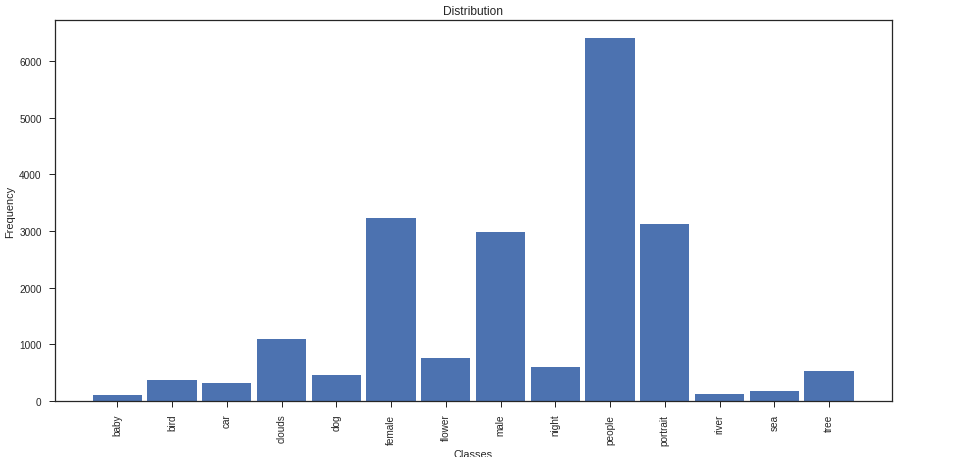
\includegraphics[width=0.6\linewidth]{images/distribution}
		\caption{Distribution of the classes}
		\label{fig:distribution-classes}
	\end{center}
\end{figure}

The main consequence of this problem is that the network could have difficulties to predict correctly the classes with a few examples in the training set. 
First we tried to penalize the loss function accordingly to the number of samples for each class by using a \textit{weights vector}. However, this didn't produce a good result.
Secondly, we tried to find a good threshold for the predictions. Each model that we tried has as final output a fully connected layer with 14 neurons (because we have 14 different classes). The activation function used in this layer is the sigmoid. So, finding the right threshold helps the model out to find the correct labels for each sample. The idea was to request a minor activation for neurons that represent classes with few examples. Vice versa for the classes with many examples. \\
We started considering as a good threshold the proportion of the data in the training set. For example, if the class 'bird' is the label of the 30\% of the dataset, the started threshold for that class is 0.3 (so to predict 1 for this class the output of the neuron should be higher respect to this value). After that we have adjusted a bit this threshold in order to have better precision than recall. Our idea was to make the predictions when there is a high activation of the corresponding neuron.

\subsection{Batching, scaling and hyperparameters}

We divided the data in this way: 90\% of the data for the training and 10\% for the validation set. We used a batch size of 64 images. We chose 64 for the following reasons. First, since we have 180000 images, having this batch size allows us to have enough updates for each epoch to get low the loss function. Second, a batch size too small would make the training really slow and variable. Finally, a bigger batch size lead us to CUDA memory problems.
The \textbf{learning rate} is chosen automatically by the \textbf{Adam optimizer}. We didn't change it because the results were good.
Finally, we added some transformations to the images - when they are taken only from the training set - to improve the results (e.g. RandomHorizontalFlip and RandomRotation).

\subsection{Splitting strategy}

To have trustable results we split the data in training and validation set making sure that each set contains the same proportion of samples for each class. Further information can be found in \texttt{image\_project\_pytorch.ipynb}.